\documentclass[11pt,a4paper]{article}

\usepackage[a4paper,margin=21mm,headheight=24pt]{geometry}
\usepackage{fontspec}
\usepackage[table]{xcolor}
\usepackage{microtype}
\usepackage{booktabs}
\usepackage{tabularx}
\usepackage{enumitem}
\usepackage{listings}
\usepackage{fancyhdr}
\usepackage{titlesec}
\usepackage{tikz}
\usetikzlibrary{positioning}
\usepackage[most]{tcolorbox}
\usepackage{hyperref}

\setmainfont{DejaVu Sans}
\setsansfont{DejaVu Sans}
\setmonofont{DejaVu Sans Mono}[Scale=0.87]

\definecolor{ink}{HTML}{172033}
\definecolor{muted}{HTML}{5E6A7D}
\definecolor{blue}{HTML}{245EA6}
\definecolor{bluepale}{HTML}{EAF2FC}
\definecolor{orange}{HTML}{B45B27}
\definecolor{orangepale}{HTML}{FFF1E8}
\definecolor{green}{HTML}{16755D}
\definecolor{line}{HTML}{D9E0EA}
\definecolor{paper}{HTML}{F7F9FC}

\hypersetup{
  colorlinks=true,
  linkcolor=blue,
  urlcolor=blue,
  pdftitle={JessiePage User Manual},
  pdfauthor={JessiePage project}
}

\pagestyle{fancy}
\fancyhf{}
\lhead{\textcolor{muted}{JessiePage User Manual}}
\rhead{\textcolor{muted}{\nouppercase{\leftmark}}}
\cfoot{\textcolor{muted}{\thepage}}
\renewcommand{\headrulewidth}{0.4pt}
\renewcommand{\headrule}{\hbox to\headwidth{\color{line}\leaders\hrule height \headrulewidth\hfill}}

\titleformat{\section}{\Large\bfseries\color{ink}}{\thesection}{0.7em}{}
\titleformat{\subsection}{\large\bfseries\color{ink}}{\thesubsection}{0.7em}{}
\titlespacing*{\section}{0pt}{2.0em}{0.8em}
\titlespacing*{\subsection}{0pt}{1.5em}{0.55em}

\setlist[itemize]{leftmargin=1.4em,itemsep=0.25em,topsep=0.35em}
\setlist[enumerate]{leftmargin=1.6em,itemsep=0.35em,topsep=0.35em}
\setlength{\parindent}{0pt}
\setlength{\parskip}{0.55em}

\lstdefinestyle{jessie}{
  basicstyle=\ttfamily\small,
  keywordstyle=\color{blue}\bfseries,
  commentstyle=\color{green},
  stringstyle=\color{orange},
  backgroundcolor=\color{paper},
  frame=single,
  rulecolor=\color{line},
  framesep=6pt,
  xleftmargin=0pt,
  breaklines=true,
  breakatwhitespace=false,
  showstringspaces=false,
  columns=fullflexible,
  keepspaces=true,
  upquote=true,
  morecomment=[l]{//},
  morestring=[b]',
  morestring=[b]",
  keywords={point,line,segment,circle,polygon,midpoint,intersection,perpendicular,circumcircle,glider,tangent,slider,functiongraph,curve,text,angle,map,solve,simplify,expand,differentiate,integrate,limit,sum,product,factor,together,numeric,substitute,range,zip,assume,forget,plot}
}

\newtcolorbox{tipbox}[1][Tip]{
  colback=bluepale,colframe=blue,boxrule=0.6pt,arc=2pt,
  title=\textbf{#1},fonttitle=\small,coltitle=ink,
  left=8pt,right=8pt,top=5pt,bottom=5pt
}
\newtcolorbox{notebox}[1][Important]{
  colback=orangepale,colframe=orange,boxrule=0.6pt,arc=2pt,
  title=\textbf{#1},fonttitle=\small,coltitle=ink,
  left=8pt,right=8pt,top=5pt,bottom=5pt
}

\newcommand{\ui}[1]{\textsf{\textbf{#1}}}
\newcommand{\code}[1]{\texttt{#1}}

\begin{document}

\begin{titlepage}
  \pagecolor{paper}
  \color{ink}
  \vspace*{24mm}
  {\fontsize{34}{40}\selectfont\bfseries JessiePage\par}
  \vspace{3mm}
  {\fontsize{19}{25}\selectfont User Manual\par}
  \vspace{12mm}
  {\large Text-first interactive geometry and computer algebra\par}

  \vfill
  
\begin{tikzpicture}
    \fill[blue,rounded corners=3pt] (0,0) rectangle (7.2,3.7);
    \fill[white,rounded corners=2pt] (0.35,0.35) rectangle (3.55,3.35);
    \fill[bluepale,rounded corners=2pt] (3.8,0.35) rectangle (6.85,3.35);
    \draw[line width=1.2pt,orange] (4.3,1.05) -- (6.35,2.6);
    \draw[line width=1.2pt,blue] (4.2,2.75) .. controls (5.0,1.3) and (5.7,3.0) .. (6.45,1.25);
    \foreach \y/\w in {2.85/2.2,2.35/1.5,1.85/2.6,1.35/1.9,0.85/2.35}
      \fill[muted!70] (0.7,\y) rectangle (0.7+\w,\y+0.08);
  \end{tikzpicture}

  \vfill
  {\small\color{muted}
    Web application: \href{https://mrsmkl.github.io/jessiepage/}{mrsmkl.github.io/jessiepage}\par
    Manual generated from the JessiePage feature set.\par
  }
  \vspace{8mm}
\end{titlepage}
\nopagecolor

\begingroup
\setlength{\parskip}{0pt}
\small
\tableofcontents
\endgroup
\clearpage

\section{What JessiePage is}

JessiePage combines two mathematical tools in one continuous text document:

\begin{itemize}
  \item \textbf{JessieCode with JSXGraph} constructs interactive points, lines, circles, polygons, curves, sliders, and other geometry.
  \item \textbf{CortexJS Compute Engine} evaluates algebra, equations, calculus, matrices, collections, and finite sums or products.
\end{itemize}

The left side is always ordinary editable text. Results are typeset beside the source line that produced them. Graphable CAS results have a small \ui{Graph} switch; enabled results share the large canvas on the right.

There are no notebook cells and no formula editor. A line is interpreted automatically from its syntax.

\subsection{The workspace}

\begin{center}
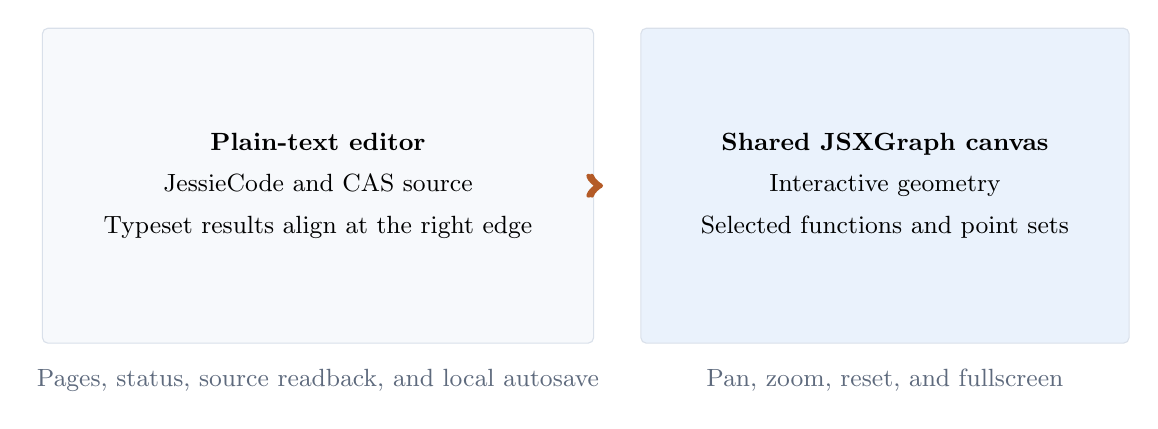
\begin{tikzpicture}[font=\small]
  \node[draw=line,fill=paper,rounded corners=2pt,minimum width=7.0cm,minimum height=4.0cm,align=center] (editor) at (0,0) {\textbf{Plain-text editor}\\[4pt] JessieCode and CAS source\\[4pt] Typeset results align at the right edge};
  \node[draw=line,fill=bluepale,rounded corners=2pt,minimum width=6.2cm,minimum height=4.0cm,align=center] (board) at (7.2,0) {\textbf{Shared JSXGraph canvas}\\[4pt] Interactive geometry\\[4pt] Selected functions and point sets};
  \draw[orange,line width=2pt,<->] (3.58,0) -- (3.62,0);
  \node[below=2mm of editor.south, text=muted] {Pages, status, source readback, and local autosave};
  \node[below=2mm of board.south, text=muted] {Pan, zoom, reset, and fullscreen};
\end{tikzpicture}
\end{center}

\section{First construction}

Open JessiePage and create or select a page. Enter the following program:

\begin{lstlisting}[style=jessie]
A = point(-3, -1);
B = point(3, -1);
C = point(0, 3);
triangle = polygon(A, B, C);
M = midpoint(A, B);
c = circle(M, C);
\end{lstlisting}

JessieCode statements normally end with a semicolon. Named objects can be reused by later statements. Editing a valid line rebuilds the construction automatically.

\subsection{Changing appearance}

JessieCode attributes follow an object in a double-angle block:

\begin{lstlisting}[style=jessie]
AB = segment(A, B) <<strokeWidth: 3, strokeColor: '#245ea6'>>;
c = circle(M, C) <<dash: 2, strokeColor: '#b45b27'>>;
triangle = polygon(A, B, C)
  <<fillColor: '#dbeafe', fillOpacity: 0.35>>;
\end{lstlisting}

Use the built-in example pages as working syntax references. They are ordinary editable programs rather than locked demonstrations.

\section{Working with the canvas}

\begin{itemize}
  \item Drag an empty area of the canvas to pan.
  \item Use the mouse wheel or a two-finger pinch to zoom.
  \item Use \ui{+} and \ui{-} on the canvas for stepped zoom.
  \item Use \ui{100\%} to restore the page's saved view.
  \item Use the canvas fullscreen control to focus on the construction.
  \item Drag the divider between editor and canvas to resize the two areas.
\end{itemize}

\subsection{Dragging points and source readback}

A point written with two literal numeric coordinates is source-backed:

\begin{lstlisting}[style=jessie]
A = point(-2, 1);
\end{lstlisting}

Dragging this point updates those coordinates in the text. The \ui{Points} area also lists the current coordinates of named points and gliders.

Constructed points are intentionally not rewritten. For example, the source of a midpoint or a point defined by \code{map () -> ...} remains the construction rule, not its temporary position.

\begin{tipbox}[Stable constructions]
Use ordinary points for inputs that students should drag. Use midpoints, intersections, gliders, and map-defined points for derived objects. This keeps the source readable and preserves the construction logic.
\end{tipbox}

\section{Pages, saving, and links}

The page selector contains user pages, general examples, Euclid postulates, common notions, and Book I propositions.

\begin{itemize}
  \item Press the top-bar \ui{+} to create a new page.
  \item Edit the page name directly in the top bar.
  \item Source, page names, selected CAS graphs, and canvas views are saved automatically in browser local storage.
  \item Press \ui{Link} to open a shareable URL containing the current program and graph selections.
\end{itemize}

\begin{notebox}[Local storage is not cloud storage]
Saved pages remain in the current browser profile. Clearing site data removes them. A shared link carries one program in its URL, but does not upload the rest of the page collection.
\end{notebox}

\section{CAS basics}

CAS expressions do not need semicolons. Definitions share one scope from top to bottom:

\begin{lstlisting}[style=jessie]
f = x^3 + 2*x^2 - x + 4
g = differentiate(f, x)
h = differentiate(g, x)
simplify(h)
\end{lstlisting}

The rendered result for each executable CAS line appears at its right. A thin connector follows the end of the source toward the result.

\subsection{Core operations}

\rowcolors{2}{paper}{white}
\begin{tabularx}{\textwidth}{@{}>{\ttfamily}l X@{}}
\toprule
\normalfont\textbf{Operation} & \textbf{Meaning} \\
\midrule
simplify(expr) & Apply general simplification. \\
expand(expr) & Expand products and powers. \\
factor(expr, x) & Factor an expression, optionally with respect to a variable. \\
together(expr) & Combine rational terms over a common denominator. \\
evaluate(expr) & Evaluate exactly where possible. \\
numeric(expr, digits) & Request a numerical approximation and optional precision. \\
substitute(expr, x, value) & Replace a variable and evaluate the result. \\
solve(expr, x) & Solve an expression equal to zero, or solve an equation. \\
differentiate(expr, x) & Differentiate with respect to a variable. \\
integrate(expr, x) & Compute an indefinite integral. \\
integrate(expr, x, a, b) & Compute a definite integral. \\
limit(expr, x, value) & Compute a limit. \\
\bottomrule
\end{tabularx}

\subsection{Equations and solutions}

\code{solve()} accepts either an equation or an expression interpreted as equal to zero:

\begin{lstlisting}[style=jessie]
f = (x - 3)*(x + 2)*(x - 1)
solve(f, x)

solve(x^2 = 9, x)
\end{lstlisting}

All representable solutions are returned as a set. Real solutions can be graphed together as points on the horizontal axis.

\section{Graphing CAS results}

If a CAS result is a function of one variable, a coordinate pair, a complex number, or a set of coordinate pairs, JessiePage offers a \ui{Graph} switch beside it.

\begin{lstlisting}[style=jessie]
f = cos(x)
g = e^x
f + g
f*g
points = {(-3,2),(-1,-2),(1,3),(3,1)}
\end{lstlisting}

Enable several switches to compare all selected results on the same axes. Each function is compiled once before JSXGraph samples it, which keeps pan and zoom responsive.

Use \code{plot(f)} only when graph activation should be part of persisted or shared source:

\begin{lstlisting}[style=jessie]
f = x^2 - 4
plot(f)
\end{lstlisting}

\subsection{Sampled points}

The collection helpers can create a complete point set from one function definition:

\begin{lstlisting}[style=jessie]
f = x^2 - 4
xs = range(-3, 3)
ys = map(f, xs)
samples = zip(xs, ys)
\end{lstlisting}

Enable the graph for \code{samples} to draw all pairs together.

\section{Plain text and LaTeX-style input}

Common function notation works as ordinary text:

\begin{lstlisting}[style=jessie]
f = sin(x) + cos(x)
g = e^x
sqrt(2)
\end{lstlisting}

LaTeX-style expressions can be mixed into the same source:

\begin{lstlisting}[style=jessie]
f = \frac{x^2}{2}
g = \sin(x)
f + g
\cos(x)
\end{lstlisting}

The source remains plain text even when the displayed result is typeset. This makes copying, editing, and versioning predictable.

\section{Finite sums and products}

JessiePage supplies plain-text wrappers because CortexJS's native function-call parser does not interpret the words \code{sum} and \code{product} as these operations by itself:

\begin{lstlisting}[style=jessie]
term = x^k
s = sum(term, k, 1, 4)
sum(k^2, k, 1, 10)

factor = x + k
p = product(factor, k, 1, 3)
product(k, k, 1, 6)
\end{lstlisting}

The equivalent LaTeX notation is also accepted directly:

\begin{lstlisting}[style=jessie]
\sum_{k=1}^{10} k
\prod_{k=1}^{6} k
\end{lstlisting}

If a finite result still contains exactly one free variable, it receives a graph switch. For example, \code{sum(x\textasciicircum{}k, k, 1, 4)} becomes a polynomial in \code{x}.

\section{Matrices, complex numbers, and assumptions}

\subsection{Matrices}

Matrices use nested lists:

\begin{lstlisting}[style=jessie]
A = [[1,2],[3,4]]
determinant(A)
inverse(A)
transpose(A)

B = [[2,1],[1,2]]
eigenvalues(B)
\end{lstlisting}

Matrix results are typeset as matrices and are not mistaken for sets of points.

\subsection{Complex numbers}

Use \code{i} for the imaginary unit:

\begin{lstlisting}[style=jessie]
z = 3 + 2*i
w = (1-i)*z
z
w
\end{lstlisting}

A non-real complex result can be graphed as \code{(real, imaginary)} on the shared canvas.

\subsection{Assumptions}

Assumptions affect subsequent CAS lines until forgotten:

\begin{lstlisting}[style=jessie]
assume(x > 0)
simplify(\sqrt{x^2})
forget(x)
simplify(\sqrt{x^2})
\end{lstlisting}

\section{Sharing variables with JessieCode}

Compatible constant values are defined in both systems. This lets one number control algebra and geometry:

\begin{lstlisting}[style=jessie]
scale = 2
offset = 1
height = scale + offset

A = point(-scale, offset);
B = point(scale, height);
segment(A, B);

f = x^2 + height
\end{lstlisting}

Numbers, booleans, and numeric collections cross from CAS into JessieCode when they have a safe representation. Multi-letter names such as \code{scale} and \code{offset} are substituted as whole identifiers rather than being split into products of letters.

\subsection{Geometry passed to the CAS}

Straightforward Jessie geometry receives a mathematical CAS representation:

\rowcolors{2}{paper}{white}
\begin{tabularx}{\textwidth}{@{}l X@{}}
\toprule
\textbf{Jessie object} & \textbf{CAS representation} \\
\midrule
Point & Coordinate pair. \\
Line & Implicit line equation in \code{x} and \code{y}. \\
Segment & Equation of the infinite carrier line; endpoint bounds are not included. \\
Circle & Implicit circle equation. \\
Quoted function graph & Equation of the form \(y=f(x)\). \\
\bottomrule
\end{tabularx}

This permits later symbolic operations:

\begin{lstlisting}[style=jessie]
A = point(-2, 0);
B = point(2, 2);
carrier = line(A, B);
solve(carrier, y)

c = circle(A, 3);
solve(c, y)
\end{lstlisting}

When a simple source-backed point moves, its dependent CAS equations refresh after the point is released.

\begin{notebox}[Deliberate limits]
Polygons, gliders, sliders, arbitrary dynamic maps, Jessie object aliases, and object collections are not forced into CAS expressions. They stay in JessieCode because a single algebraic value would be incomplete or misleading.
\end{notebox}

\section{Euclid Book I}

The built-in Euclid collection contains:

\begin{itemize}
  \item the five postulates;
  \item the five common notions; and
  \item all 48 propositions of Book I.
\end{itemize}

Each page is an editable JessieCode construction. Movable inputs are ordinary points wherever practical, so dragging them can update their coordinates in the source. Captions and numerical statements use dynamic text when the geometry changes.

The diagrams are intended as interactive illustrations of the constructions and claims. The postulates and common notions are assumptions, and the diagrams are not substitutes for Euclid's proofs.

\section{Errors and troubleshooting}

\subsection{A line shows a CAS error}

Check parentheses, braces, argument count, and variable spelling. CAS errors are attached to their source line and do not prevent later independent CAS lines from being analyzed.

\subsection{A Jessie construction does not redraw}

JessieCode statements generally require semicolons. Check the highlighted error line, then compare the syntax with a built-in geometry example.

\subsection{A result has no Graph switch}

The value may be scalar, a matrix, a relation, a function of more than one free variable, or another result without an unambiguous two-dimensional graph. Use substitution or solve for one variable first.

\subsection{Typing or navigation feels slow}

Keep functions in shared definitions instead of repeating large expressions. Graph callbacks are compiled once, but extremely large symbolic results can still be expensive. Turn off graphs that are not currently needed.

\subsection{A saved page disappeared}

Pages are stored in the browser profile. Check whether site data was cleared, private browsing was used, or a different browser/profile is open. Use \ui{Link} for individual programs that need a portable copy.

\section{Compact reference}

\subsection{Common JessieCode constructors}

\begin{tabularx}{\textwidth}{@{}>{\ttfamily}l X@{}}
\toprule
\normalfont\textbf{Constructor} & \textbf{Purpose} \\
\midrule
point(x,y) & Free or computed point. \\
line(A,B) & Infinite line through two points. \\
segment(A,B) & Segment between two points. \\
circle(O,A) & Circle with center \code{O} through \code{A}. \\
polygon(A,B,C,...) & Polygon with the listed vertices. \\
midpoint(A,B) & Midpoint of two points. \\
intersection(a,b,n) & Indexed intersection of two objects. \\
perpendicular(l,A) & Perpendicular to a line through a point. \\
glider(x,y,obj) & Point constrained to an object. \\
tangent(P) & Tangent determined by a glider or contact point. \\
slider(p1,p2,[min,value,max]) & Interactive numeric control. \\
functiongraph('expr') & Graph of a quoted function. \\
curve(fx,fy,t0,t1) & Parametric curve. \\
text(x,y,value) & Static or dynamic text. \\
angle(A,B,C) & Angle with vertex \code{B}. \\
\bottomrule
\end{tabularx}

\subsection{Keyboard and editing reminders}

\begin{itemize}
  \item Source is plain text and accepts ordinary copy and paste.
  \item Autocomplete suggests constructors, CAS calls, functions, and names already defined in the source.
  \item Pasting suppresses autocomplete so it cannot interfere with immediate evaluation.
  \item Results are overlays; selecting and editing the underlying source does not require entering a separate result cell.
\end{itemize}

\section{Further information}

\begin{itemize}
  \item JessiePage: \url{https://mrsmkl.github.io/jessiepage/}
  \item Source repository: \url{https://github.com/mrsmkl/jessiepage}
  \item JessieCode reference: \url{https://jsxgraph.org/docs/symbols/JXG.JessieCode.html}
  \item CortexJS Compute Engine: \url{https://cortexjs.io/compute-engine/}
\end{itemize}

\vfill
\begin{center}
  \color{muted}\small End of manual
\end{center}

\end{document}
